% STEREO
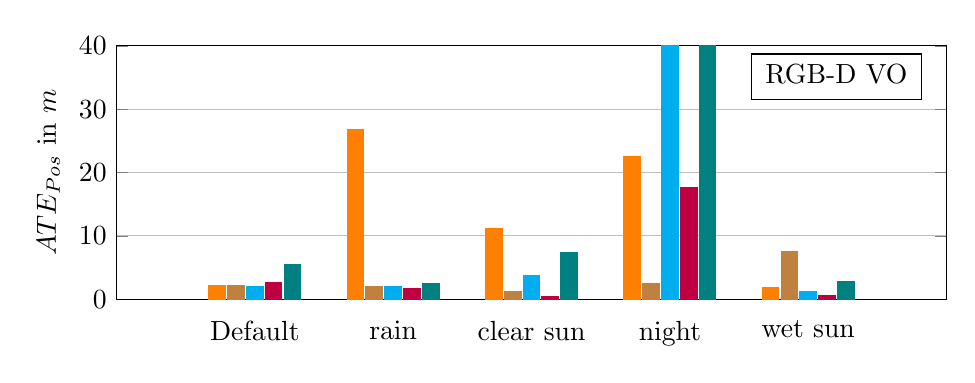
\begin{tikzpicture}
    \begin{axis}[
        width  = \textwidth,
        height = 4.8cm,
        ymax =40,
        major x tick style = transparent,
        ybar=2*\pgflinewidth,
        bar width=6pt,
        ymajorgrids = true,
        ylabel = {$ATE_{Pos}$ in $m$},
        % xlabel = {1 Default, 2 hard rain, 3 clear sunset, 4 clear night ,5 wet sunset},
        symbolic x coords={Default, rain, clear sun, night ,wet sun},
        xtick = data,
        scaled y ticks = false,
        enlarge x limits=0.25,
        ymin=0,
        legend pos=north east
    ]
    \addlegendimage{empty legend}
    \addlegendentry{RGB-D VO}

    \addplot[style={orange,fill=orange,mark=none}]
        coordinates {(Default, 2.10) (rain, 26.85) (clear sun, 11.109) (night , 22.593) (wet sun, 1.85)};
    
    \addplot[style={brown,fill=brown,mark=none}]
        coordinates {(Default, 2.16) (rain, 2.02) (clear sun, 1.28) (night , 2.518) (wet sun, 7.512)};
    
    \addplot[style={cyan,fill=cyan,mark=none}]
        coordinates {(Default, 1.94) (rain, 2.057) (clear sun, 3.768) (night , 75.997) (wet sun, 1.1535)};
    
    \addplot[style={purple,fill=purple,mark=none}]
        coordinates {(Default, 2.62) (rain, 1.648) (clear sun, 0.480) (night , 17.566) (wet sun, 0.52516)};
    
    \addplot[style={teal,fill=teal,mark=none}]
        coordinates {(Default, 5.55) (rain, 2.432) (clear sun, 7.2941) (night , 83.744) (wet sun, 2.789)};
    \end{axis}
  \end{tikzpicture}